The Silicon Photomultiplier (SiPM), also called Multi-Pixel Photon Counter (MPPC), is a kind of photosensor based on semiconductor materials, developed in the last two decades. SiPMs are replacing progresively conventional PMTs in many experiments and applications. They have outstanding photon counting capabilities at the single photon level with higher photodetection efficiency than PMT and they have similar gain. SiPMs have, in addition, several advantages as insensitiveness to magnetic fields, low operating voltage, compactness (they may have down to $1~\mm^2$) and ruggedness. The only drawback with respect to the PMTs is their high dark count rate (between $100~\kilo\hertz$ and $1~\mega\hertz$).

SiPMs are formed by a matrix of Avalanche Photodiodes (APDs) conected in parallel and operating in Geiger mode. APDs, the scheme of which is shown in Figure \ref{fig:SchemeAPD}, are based on p-n junctions\footnote{A p-n junction is a junction of a p+ and n+ layer, which are a tetravalent material doped with a trivalent or pentavalent material respectively, creating sublevels in the forbidden energy gap.} made with special techniques to achieve a good contact between both surfaces.

\begin{figure}[htbp]
\centering
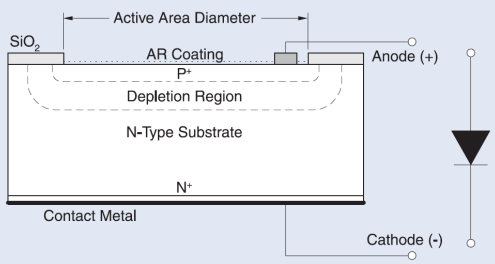
\includegraphics[scale=0.6]{3DesignPrinciples/32Tritium_detector/APD_scheme.png}
\caption{Scheme of a APD and electrical symbol used\label{fig:SchemeAPD}~\cite{OSI}.}
\end{figure}
 

The voltage at which the SiPM starts operating in Geiger mode is called the breakdown voltage, $V_ {BD}$. At lower voltages, SiPMs work in proportional mode in which the signal of each APD is proportional to the energy deposited but their gain is lower than in Geiger mode. The experimental measurement of the breakdown voltage, described in section \ref{sec:CharacterizationSiPM}, is an important measurement to characterize a SiPM, since properties of SiPMs, as the gain, depend on the overvoltage, $V_{OV}$. The overvoltage is the voltage applied to the SiPM above its breakdown voltage and this is expressed as:

\begin{equation}
V_{bias}=V_{BD}+V_{OV}
\label{overvoltage}
\end{equation}

These APDs, called pixels when they are part of a SiPM, are connected in parallel and the output signal of the SiPM is the sum of all of them. If the photon flux is low enough, each SiPM pixel detects only one photon and its output signal is similar compared to other pixels of the same SiPM, regardless of the energy deposited, with some difference because of the uncertainty due to the SiPM manufacturing process and the statistical nature of photoelectron production. Therefore, the charge of the output signal when $n$ pixels are simultaneously fired is $n$ times the charge of a single pixel, as can be checked in Figure \ref{fig:PulsesOfSiPM}. Due to this property, the number of detected photons is linearly proportional to the value of the output signal area. In addition, as the detected photons are porportional to the incident photons when the SiPM are working in the linearity range, after an accurate calibration of SiPM gain, described in section \ref{sec:CharacterizationSiPM}, the linearity of the SiPM output signal versus the number of incident photons and, therefore, the deposited energy of tritium events, is recovered.

\begin{figure}[h]
\centering
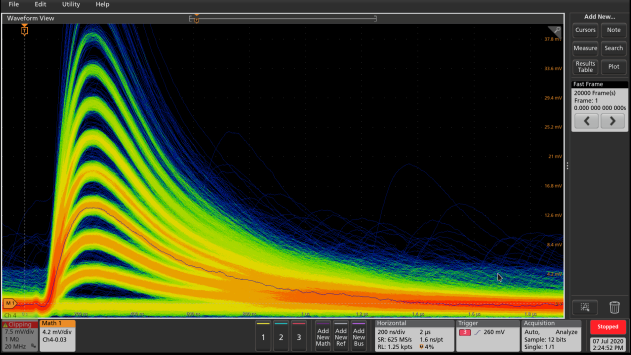
\includegraphics[scale=0.6]{3DesignPrinciples/32Tritium_detector/Several_SiPM_pulses.png}
\caption{SiPM output pulses displayed on oscilloscope, model MSO44X from Tektronix \cite{Oscilloscope}. Several height pulses are observed, associated to a different number of  SiPM pixels fired at the same time. The persistence function of the oscilloscope is used.\label{fig:PulsesOfSiPM}}
\end{figure}

If the photon flux is high (typically several thousands of photons per event) more than one photon will impinge on the same pixel, but the output signal would be that of one only detected photon. This effect, known as saturation, produces a loss of linearity of the output signal. However, this effect is not important for the TRITIUM detector since its scintillating signals are far from producing so many photons. %The experimental measurements of this effect, which have been done for our SiPMs, is shown in section \ref{sec:CharacterizationSiPM}. 

Different sizes of the SiPM pixel can be chosen\footnote{Pixel sizes for commercial SiPMs are $25$, $50$ or $75\mu\meter$ \cite{DataSheetHammamatsu_1_SiPM_25}, \cite{DataSheetHammamatsu_1_SiPM_50}, \cite{DataSheetHammamatsu_1_SiPM_75}}. For the same active area of the SiPM, the smaller pixels allow the SiPM to have more pixels, which implies a higher dynamic range, at the cost of reducing its quantum efficiency. As the TRITIUM detector signals have few photons, the SiPMs used have the largest pixel size as we are far from the limit of dynamic range and quantum efficiency is a critical parameter for tritium detection.

%The size of a SiPM pixel should be very small\footnote{Pixel sizes for commercial SiPMs are $25$, $50$ or $75\mu\meter$ \cite{DataSheetHammamatsu_1_SiPM_25}, \cite{DataSheetHammamatsu_1_SiPM_50}, \cite{DataSheetHammamatsu_1_SiPM_75}} to make sure that, for low enough photon fluxes, only one photon is detected in each pixel.

The SiPM can be modeled as an electric circuit, shown in figure \ref{subfig:ElectricModelSiPM}, in which, due to the charge distribution in the depletion zone, a capacitance is induced by the SiPM. This is schematized as a reverse biased diode in parallel with a capacitor of capacitance $C_d$, as shown in Figure \ref{subfig:ElectricModelSiPM}. When the pixel detects a photon, the capacitor is discharged, creating an output current (electronic pulse).

In addition, each pixel of a SiPM has a quenching resistance\footnote{The tipical value of this quenching resistance for commercial SiPMs is around $500~\kilo\Omega$} in serie, $R_q$, that stops the avalanche current produced when this pixel is fired, creating a time limited electronic pulse. When the discharge is produced, a current flows through the resistance, reducing the reverse voltage seen by the diode below the breakdown voltage. Then, the current that flows through the diode is stopped and the voltage within the diode is reset to the bias voltage. This pixel is ready to detect a new photon again. This behaviour is schematically shown in Figure \ref{subfig:HowSiPMworks}.

\begin{figure}
\centering
    \begin{subfigure}[]{0.45\textwidth}
    \centering
    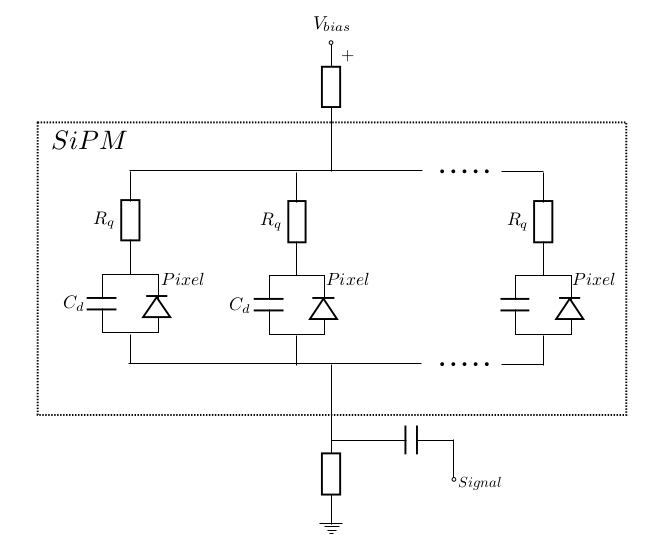
\includegraphics[width=\textwidth]{3DesignPrinciples/32Tritium_detector/SimpliestElectronicSchemeSiPM.png}  
    \caption{\label{subfig:ElectricModelSiPM}}
    \end{subfigure}
    \hfill
    \begin{subfigure}[]{0.45\textwidth}
    \centering
    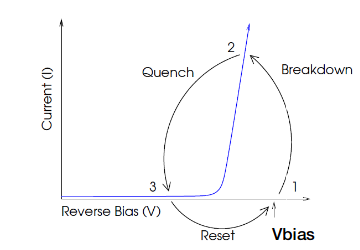
\includegraphics[width=\textwidth]{3DesignPrinciples/32Tritium_detector/How_a_quenching_resistence_in_a_SiPM_works.png}  
    \caption{\label{subfig:HowSiPMworks}}
    \end{subfigure}
 \caption{(a) Electronic scheme of a SiPM and (b) output current of a SiPM as a function of the reverse voltage. As shown, the quenching is an essential working mechanism of SiPMs~\cite{DataSheetSensL}.}
 \label{fig:ChenchingResistance}
\end{figure}

The recovery of the bias voltage within the SiPM pixel after photon detection is characteristic of a RC circuit, described by the equation: 

\begin{equation}
V_{bias}(t)=V(t_0)\left(1-e^{-t/\tau} \right)
\label{RCCircuitBiasVoltage}
\end{equation}
where $\tau$ is the recovery time constant of the system, given by $\tau=C_d \times R_q$. In section \ref{sec:CharacterizationSiPM} the capacitance $C_d$ and the quenching resistance $R_q$ are measured and the recovery time constant extrapolated from both.

SiPM gain (typically of the order of $10^6$) is defined as the number of charges produced when a single pixel is fired. This can be measured from the SiPM Single Photon Spectrum (SPS), which is the spectrum obtained when the SiPM output signal is integrated (charge) and histogrammed. The experimental measurement of the SPS and the calculation of the gain is presented in section \ref{sec:CharacterizationSiPM}. It has to be taken into account that the SiPM gain is highly dependent on temperature, which cannot be controlled with sufficient sensitivity (less than $1\celsius$) in the final location of the TRITIUM monitor. Therefore, a gain stabilization method was implemented to compensate for the temperature effect. This method is detailed in section \ref{sec:CharacterizationSiPM}.

An important parameter for the SiPM used in the TRITIUM project is the photon detection efficiency, PDE. This is defined as the probability of recording the electrical pulse produced by a photon that hit the SiPM. The PDE of a SiPM consists of a product of three different paramenters, the fill factor ($FF$), which is the ratio between the active area of the SiPM and its total area, the quantum efficiency ($QE$), which is the probability of producing a photoelectron when a photon hits the SiPM and the probability that the generated electron or hole produces an avalanche, $P_{av}$.

\begin{equation}
PDE=FF \times QE \times P_{av}
\label{PDE_SiPM}
\end{equation}

Likewise PMTs, SiPMs produce pulses that are unrelated with any incident photon, called the dark current. The pulse rate of these events is called dark current rate and it depends on temperature. At temperatures around $25\celsius$, these pulses are mainly produced by the thermal generation, i.e., when the temperature produce a thermal energy allowing electrons from the valence band to overcome the forbidden band and go up to the conduction band. The dark current signal is identical to the signal produced by a single photon, so they cannot be discriminated. Therefore, it is very important to determine the magnitude of the dark current in the tritium signal from the detector.

Electrons contained in an avalanche of a SiPM pixel emit secondary optical photons\footnote{Around 20 secondary optical photons are emitted in each SiPM output pulse with gains of the order of $10^6$ \cite{CrosstalkProbability}}. These optical photons can reach other pixels, producing new avalanches. This effect, called optical cross-talk, produces photoelectrons that add to those truly induced by incident photons, and hence leads to an overestimation of the number of photons detected. The probability of producing an optical crosstalk event depends on the number of electrons produced in the avalanche (gain) and, therefore, on the temperature and the overvoltage. This probability at the overvoltage recommended at $25\celsius$ by the manufacturer is typically less than $10\%$.

The PDE, dark count rate and crosstalk are not measured yet since a different setup, shown in reference \cite{PDEStudy}, is needed. These parameters will be measured for the SiPM model used in the final version of TRITIUM monitor.

Due to imperfections existing in the cristal lattice of a SiPM, called traps, an electron of an avalanche can be captured and released after a characteristic time, $\tau_a$. If this characteristic time is longer than the pixel recovery time, typically $3\tau$, this electron can trigger a new avalanche which will be seen as a new event. These events, called  afterpulses, are often emitted around $1~\mu\second$ after the photon-incident pulses. The afterpulse probability was not measured since it is not relevant for the TRITIUM project. The reason is that the TRITIUM detector makes time coincidences using $10~\nano\second$ time windows. At this level, the afterpulse probability is negligible since it normally happens $1~\mu\second$ after the SiPM output pulse.

The initial SiPM candidate for TRITIUM project and the one which was characterized is the model S13360-1375 from Hamamatsu Photonics \cite{DataSheetHammamatsu_1_SiPM_1375} because this model has interesting characteristics and properties, shown in Table \ref{tab:PropertiesOfSiPM1375}. This model was mainly chosen due to its large pixel size, $75~\mu\meter$, which implies a high PDE and a high gain, both important parameters for the TRITIUM project due to the low activity to be detected and to the small signals produced by tritium events. High PDE and high gain are achieved at the cost of reducing the dinamic range, which is not an issue due to the small photon signals expected from tritium events in the scintillating fibers. 

\begin{table}[htbp]
\centering{}%
\begin{tabular}{lcc}
\toprule 
Parameter & S13360-1375 & S13360-6075 \tabularnewline
\midrule
\midrule 
Series & $S13360$ & $S13360$ \tabularnewline
Model & $1375$ & $16075$ \tabularnewline
Pixel Pitch ($\mu\meter$) & $75$ & $75$ \tabularnewline
Effective photosensitive area ($\mm^2$) & $1.3 \times 1.3$ & $6.0 \times 6.0$ \tabularnewline
Number of pixels & $285$ & $6400$ \tabularnewline
Fill factor & $82\%$ & $82\%$ \tabularnewline
Refractive index of windows material & $1.55$ & $1.55$ \tabularnewline
Operating temperature range ($\celsius$) & $[-20,60]$ & $[-20,60]$ \tabularnewline
Spectral response range, $\lambda$ ($\nano\meter$) & $[320, 900]$ & $[320, 900]$ \tabularnewline
Peak sensitivity wavelength, $\lambda_p$ ($\nano\meter$) & $450$ & $450$ \tabularnewline
PhotoDetection Efficiency, PDE, $\lambda=\lambda_p$ ($\%$) & $50$ & $50$ \tabularnewline
Dark counts, Typical/Maximum (kcps) & $90/270$ & $2000/6000$ \tabularnewline
Terminal capacitance, $C_t$ ($\pico\farad$) & $60$ & $1280$ \tabularnewline
Gain, M, & $4 \cdot{} 10^6$ & $4 \cdot{} 10^6$ \tabularnewline
Breakdown Voltage, $V_{BD}$ ($\volt$) & $50.97$ & $53$ \tabularnewline
Cross talk probability($\%$) & $7$ & $7$ \tabularnewline
Temperature coefficient $\Delta TV_{op}$ (m$\volt/\celsius$) & $54$ & $54$ \tabularnewline
\bottomrule
\end{tabular}
\caption{Characteristics of SiPM S13360-1375 and S13360-6075 from Hamamatsu Photonics \cite{DataSheetHammamatsu_1_SiPM_1375}.}
\label{tab:PropertiesOfSiPM1375}
\end{table}

These parameters quoted in Table \ref{tab:PropertiesOfSiPM1375}, are typical values provided by the manufacturer, Hamamatsu photonics. They can vary significantly from one SiPM to another of the same model. Thus, it is convenient and sometimes necessary to measure them. Some of these measurements for TRITIUM are reported in section \ref{sec:CharacterizationSiPM}. 

This SiPM was also chosen because, as it can be observed in Figure \ref{fig:PDESiPM}, its maximum PDE is reached at $\lambda_{p,SiPM}=450~\nano\meter$, which is very close to the peak of the emission spectrum of the scintillating fibers used, $\lambda_{p,fiber}=435~\nano\meter$.

\begin{figure}[htbp]
\centering
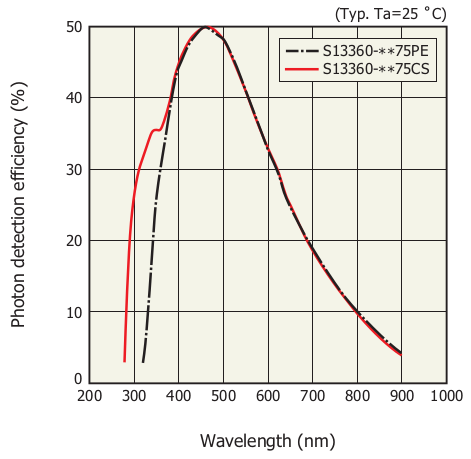
\includegraphics[scale=0.6]{3DesignPrinciples/32Tritium_detector/SiPMPDE.png}
\caption{Photon detection efficiency (PDE) spectrum for SiPM S13360-**75 models~\cite{DataSheetHammamatsu_1_SiPM_1375}.\label{fig:PDESiPM}}
\end{figure}

This SiPM was later replaced by the model S13360-6075 from Hamamatsu Photonics \cite{DataSheetHammamatsu_1_SiPM_75}, whose properties are also listed in Table \ref{tab:PropertiesOfSiPM1375}. The only difference between both models is their larger active area ($6\times6~\mm^2$), which is the largest active area of commercial SiPMs of Hamamatsu, that allows to read more scintillating fibers. This improvement is achieved at the price of a higher dark count rate (typically 2 Mcps). Finally, arrays of this SiPM model are commercially available and were chosen for the TRITIUM detector prototypes built at IFIC.

Although TRITIUM detector uses SiPM matrices, the caracterization has been carried out at the level of a single SiPM to learn about the values of the SiPM parameters and to test the gain control method. %A new experimental setup, detailed in appendix \ref{App:ElectronicReadoutSiPM}, is already  prepared to perform a complete characterization of the SiPM model S13360-6075.